\tableofcontents
\newpage
\section*{Introduction}
This is the lab report for \href{https://www.canvas.umu.se/courses/6705/assignments/75609}{Assignment 2} of \href{https://www.umu.se/en/education/courses/stochastic-processes-and-simulation/}{Stochastic processes and Simulations} during the autumn of 2022. The assignment consists of three different tasks regarding natural random processes. These tasks will be described in detail under each task section.
% Describe theoretical background of the tasks 
% Don’t forget to define all the symbols and notation used  
% The theory should not be task specific

\section{Task 1: White Rat}
\label{sec:task1}

\subsection{Task Description}
\label{sec:desc1}
A white rat is put into random cell of the maze (represented as a Markov chain in Figure \ref{fig:ratchain}) below. There are nine compartments with connections between the compartments as indicated. At each time step the rat moves through the compartments at random. That is, if there are k ways to leave a compartment, it chooses each of these with equal probability. 
\\
\\a) Consider long period of time (n=100 000 time steps). Use simulations to estimate the proportion of
time spent by the rat in each cell.
\\
\\b) Use Matlab to compute theoretical solution of the problem. Present necessary reasoning guaranteeing existence of the solution presented.
\\
\\c) Assume now that a rat is placed in the position 5 initially (at time 0). Based on 1000 trials, what is
the estimate of the expected time for the rat to return to its initial position? What is the standard error associated with your point estimate?

\begin{figure}[H]
    \centering
    \markovchain{}
    \caption{Visualization of the Markov chain constructed from the given conditions of equal probability of leaving to each adjacent cell. The values on each outgoing edge of the graph represents the probability that the rat chooses to travel via that edge.}
    \label{fig:ratchain}
\end{figure}



%Copy of the task description
\newpage
\subsection{Theory}
\label{sec:theory1}

The theory used in this exercise can be found in the lecture slides regarding Markov Chains.

\subsubsection{Markov Chains}
\label{sec:markov1}

\begin{definition}{(Markov Chains)}
    A Markov Chain is a stochastic model that describes a sequence(chain) of possible events. The different events probability depend only on the previous state which can be expressed as
\begin{equation}
    P(X_{n+1} = j|X_n = i,X_{n-1} = i_1,...) = P(X{n+1} = j|X_n = i) = p_{ij}
\end{equation}
$p_{ij}$ is the probability going from i to j are called transition probabilities.
\end{definition}

\begin{figure}[H]
    \centering
    \triangles{}
    \caption{Figure 1 represents a simple Markov Chain and its corresponding transition probabilities.}
\end{figure}


The probabilities can also be arranged into the following matrix:

\begin{equation*}
P = 
\begin{bmatrix}
a_{11} & a_{12} & \cdots & a_{1N} \\
a_{21} & a_{22} & \cdots & a_{2N} \\
\vdots  & \vdots  &  & \vdots  \\
a_{N1} & a_{N2} & \cdots & a_{NN} 
\end{bmatrix}
\end{equation*}
The row index corresponds to the state of chain at time n, and
the column corresponds to the state in time n + 1. The total sum of each row has to equal to 1 since there has to be a transition.
\begin{equation}
    \sum_{j=1}^{N} p_{ij} = 1
\end{equation}
The different types of Markov Chains are Irreducible Markov Chains:

\begin{definition}{(Irreducible Markov Chain)}{irreducible}

The Markov Chain $X_n,n = 0,1,2,...$ with space state $\{1,2,...,N\}$
is called irreducible if each state $j,j \in \{1,2,...,N\}$ can be
reached in a finite time from any other state.
\end{definition}

And Aperiodic Markov Chains:

\begin{definition}{(Aperiodic Markov Chains)} 
\ The Markov Chain $X_n,n = 0,1,2,...$ with space state $\{1,2,...,N\}$
is aperiodic if for all states $j,j \in \{1,2,...,N\}$ there exists n such that \begin{equation}
    P(X_n = j|X_0 = j) >0 \ and \  P(X_{n+1} = j|X_0 = j) >0
\end{equation}
\end{definition}

\begin{theorem}{(Asymptotic distribution)}
    :Let $X_n,n = 0,1,2,...$ with space state $\{1,2,...,N\}$ be an
irreducible and aperiodic Markov Chain. Then there exist an asymptotic distribution $\pi=(\pi_1,\pi_2,...,\pi_N)$ Such that 

\begin{equation}
    \lim_{n \to\infty} P(X_n = j|X_0 = i) = \pi_j\ Independently\ of\ i,
\end{equation}
or terms of transition matrix

\begin{equation}
    \lim_{n \to\infty} P^n = \begin{bmatrix}
\pi_1 & \pi_2 & \cdots & \pi_N \\
\pi_1 & \pi_2 & \cdots & \pi_N \\
\vdots  & \vdots  &  & \vdots  \\
\pi_1 & \pi_2 & \cdots & \pi_N 
\end{bmatrix}
\end{equation}
\end{theorem}

% Describe theoretical background of the tasks 
% Don’t forget to define all the symbols and notation used  sied0020
% The theory should not be task specific



\subsection{Method}
\label{sec:method1}

% Here you describe how you use the theory introduced to solve the task. 
% Define clearly relationship between your problem  and theory. This includes introducing notation and assigning it to your problem. 
% If there is need for any analytical calculations you should present them here (calculations of theoretical task, finding constants or other parameters of your algorithm)

In our task the transition matrix is given by
\begin{equation*}
 P = 
\begin{bmatrix}
          0 &    1/2       &   0       &   0      &    0  &   1/2        &  0  &        0       &   0 \\
     1/3    &     0  &  1/3     &    0 &   1/3      &   0&         0        & 0        & 0 \\
          0 &    1/2         & 0   & 1/2       &  0       &  0        & 0        & 0  &       0 \\
          0 &         0  &  1/3       &  0   & 1/3       &  0       &  0       &  0  &  1/3 \\
          0 &    1/4       &  0  &  1/4   &      0  &  1/4       &  0  &  1/4  &       0 \\
     1/3 &         0       &  0       &  0  &  1/3   &      0  &  1/3       &  0  &       0 \\
          0 &         0  &       0       &  0       &  0  &  1/2       &  0  &  1/2  &       0 \\
          0 &         0       &  0       &  0   & 1/3       &  0  &  1/3       &  0  &  1/3 \\
          0 &         0     &    0   & 1/2       &  0        & 0       &  0  &  1/2  &       0 
\end{bmatrix}
\end{equation*}
and a position is given by a 9-element row vector $p$ with zeros everywhere except for a single index where there is a one. 

We notice that our Markov chain is irreducible since we can reach all positions from everywhere. 

We also see that it is periodic. Since we always need an even number of steps (as many steps up as down, and as many left as right) to get back to the place we started, we can never reach it in two consecutive time steps.

\subsubsection{Algorithm A}
\label{sec:alg1A}

For $N = 100\ 000$ we repeatedly update the position of an initially randomly placed rat. Each time the rat is put in a cell we update a counter for this cell, so that we after having run all the updates can compute the fraction of the time spent in each cell. This procedure is shown in Algorithm \ref{alg:1A}.

\begin{algorithm}[H]
    \label{alg:1A}
    \caption{Simulate proportion of time spent in each cell.}
    $counter \gets (0, 0, 0, 0, 0, 0, 0, 0, 0)$ \;
    $p \gets rand(1:9)$ \;
    \For{$i \in 1:N$}{
        $pos \gets (0, 0, 0, 0, 0, 0, 0, 0, 0)$ \;
        $pos(p) \gets 1$ \;
        $counter(p) \gets counter(p) + 1$ \;
        $pos \gets pos * P$ \;
        $p \gets InverseTransform(pos)$ \;
    }
    $fraction \gets \frac{1}{N} * counter$
\end{algorithm}

After running this, the $fraction$ will contain a vector of the proportion of time spent in each cell.
\\ 

The \textit{InverseTransform} function is a function which returns an index to the input vector with proportion equal to the probabilities in it.
This is done using the inverse transform algorithm for discrete distributions. See Algorithm \ref{alg:IT}.

\begin{algorithm}[H]
    \label{alg:IT}
    \caption{Inverse Transform given discrete probabilities.}
    \KwInput{$density$ A vector of probabilities for each position.}
    \KwOutput{$i$ An index selected with probability proportional as to what is given in the $density$.}
    \Fn{$InverseTransform(density)$}{
        $U \sim \mathcal{U}(0,1)$ \Comment*{Uniformly distributed random number}
        $p \gets 0$ \;
        $i \gets 0$ \;
        \While{$p < U$}{
            $i \gets i + 1$\;
            $p \gets p + density[i]$\;
        }
        
        \Return $i$
    }
\end{algorithm}


\subsubsection{Algorithm B}
\label{sec:alg1B}

We set up the equation system and let \texttt{Matlab} solve it for us. 

The equations will be (as a linear equation system): 

\begin{equation*}
\begin{bmatrix}
  \pi_1 \\  \pi_2 \\  \pi_3 \\  \pi_4 \\  \pi_5 \\  \pi_6 \\  \pi_7 \\  \pi_8 \\  \pi_9 
\end{bmatrix}^T
%\begin{bmatrix} % SPARA DETTA
%          0 &    1/2       &   0       &   0      &    0  &   1/2        &  0  &        0       &   0 \\
%     1/3    &     0  &  1/3     &    0 &   1/3      &   0&         0        & 0        & 0 \\
%          0 &    1/2         & 0   & 1/2       &  0       &  0        & 0        & 0  &       0 \\
%          0 &         0  &  1/3       &  0   & 1/3       &  0       &  0       &  0  &  1/3 \\
%          0 &    1/4       &  0  &  1/4   &      0  &  1/4       &  0  &  1/4  &       0 \\
%     1/3 &         0       &  0       &  0  &  1/3   &      0  &  1/3       &  0  &       0 \\
%          0 &         0  &       0       &  0       &  0  &  1/2       &  0  &  1/2  &       0 \\
%          0 &         0       &  0       &  0   & 1/3       &  0  &  1/3       &  0  &  1/3 \\
%          0 &         0     &    0   & 1/2       &  0        & 0       &  0  &  1/2  &       0 \\ 
%          1 & 1 & 1 & 1 & 1 & 1 & 1 & 1 & 1 
%\end{bmatrix} % OSKAR, tror det var nog fel håll på ettorna, bytte till en kolumn full med ettor, samt höger byta ut pi_9 mot 1 motför lägga till 1 längst ned 
% hmm - i matlab-koden har vi P-I ist med, innan vi byter ut ettorna!
% SPARA DETTA
\begin{bmatrix}
          0 &    1/2       &   0       &   0      &    0  &   1/2        &  0  &        0       &   0 \\
     1/3    &     0  &  1/3     &    0 &   1/3      &   0&         0        & 0        & 0 \\
          0 &    1/2         & 0   & 1/2       &  0       &  0        & 0        & 0  &       0 \\
          0 &         0  &  1/3       &  0   & 1/3       &  0       &  0       &  0  &  1/3 \\
          0 &    1/4       &  0  &  1/4   &      0  &  1/4       &  0  &  1/4  &       0 \\
     1/3 &         0       &  0       &  0  &  1/3   &      0  &  1/3       &  0  &       0 \\
          0 &         0  &       0       &  0       &  0  &  1/2       &  0  &  1/2  &       0 \\
          0 &         0       &  0       &  0   & 1/3       &  0  &  1/3       &  0  &  1/3 \\
          0 &         0     &    0   & 1/2       &  0        & 0       &  0  &  1/2  &       0 \\ 
\end{bmatrix}
= 
%\begin{bmatrix} % SPARA DETTA
%  \pi_1 \\  \pi_2 \\  \pi_3 \\  \pi_4 \\  \pi_5 \\  \pi_6 \\  \pi_7 \\  \pi_8 \\  \pi_9 \\ 1
%\end{bmatrix}^T % SPARA DETTA
\begin{bmatrix}
  \pi_1 \\  \pi_2 \\  \pi_3 \\  \pi_4 \\  \pi_5 \\  \pi_6 \\  \pi_7 \\  \pi_8 \\  pi_9\\
\end{bmatrix}^T
\end{equation*}

Which implies $\pi P - \pi = \pi (P - 1) = 0$. We can also replace one column because of the requirement that the probabilities should add to 0; $\sum^9_{i=1} \pi_i = 1$.

\begin{equation*}
\begin{bmatrix}
  \pi_1 \\  \pi_2 \\  \pi_3 \\  \pi_4 \\  \pi_5 \\  \pi_6 \\  \pi_7 \\  \pi_8 \\  \pi_9 
\end{bmatrix}^T
%\begin{bmatrix} % SPARA DETTA
%          0 &    1/2       &   0       &   0      &    0  &   1/2        &  0  &        0       &   0 \\
%     1/3    &     0  &  1/3     &    0 &   1/3      &   0&         0        & 0        & 0 \\
%          0 &    1/2         & 0   & 1/2       &  0       &  0        & 0        & 0  &       0 \\
%          0 &         0  &  1/3       &  0   & 1/3       &  0       &  0       &  0  &  1/3 \\
%          0 &    1/4       &  0  &  1/4   &      0  &  1/4       &  0  &  1/4  &       0 \\
%     1/3 &         0       &  0       &  0  &  1/3   &      0  &  1/3       &  0  &       0 \\
%          0 &         0  &       0       &  0       &  0  &  1/2       &  0  &  1/2  &       0 \\
%          0 &         0       &  0       &  0   & 1/3       &  0  &  1/3       &  0  &  1/3 \\
%          0 &         0     &    0   & 1/2       &  0        & 0       &  0  &  1/2  &       0 \\ 
%          1 & 1 & 1 & 1 & 1 & 1 & 1 & 1 & 1 
%\end{bmatrix} % OSKAR, tror det var nog fel håll på ettorna, bytte till en kolumn full med ettor, samt höger byta ut pi_9 mot 1 motför lägga till 1 längst ned 
% hmm - i matlab-koden har vi P-I ist med, innan vi byter ut ettorna!
% SPARA DETTA
\begin{bmatrix}
          -1 &    1/2       &   0       &   0      &    0  &   1/2        &  0  &        0       &   1 \\
     1/3    &     -1  &  1/3     &    0 &   1/3      &   0&         0        & 0        & 1 \\
          0 &    1/2         & -1   & 1/2       &  0       &  0        & 0        & 0  &       1 \\
          0 &         0  &  1/3       &  -1   & 1/3       &  0       &  0       &  0  &  1 \\
          0 &    1/4       &  0  &  1/4   &      -1  &  1/4       &  0  &  1/4  &       1 \\
     1/3 &         0       &  0       &  0  &  1/3   &      -1  &  1/3       &  0  &       1 \\
          0 &         0  &       0       &  0       &  0  &  1/2       &  -1  &  1/2  &       1 \\
          0 &         0       &  0       &  0   & 1/3       &  0  &  2/3       &  -1  &  1 \\
          0 &         0     &    0   & 1/2       &  0        & 0       &  0  &  1/2  &       1 \\ 
\end{bmatrix}
= 
%\begin{bmatrix} % SPARA DETTA
%  \pi_1 \\  \pi_2 \\  \pi_3 \\  \pi_4 \\  \pi_5 \\  \pi_6 \\  \pi_7 \\  \pi_8 \\  \pi_9 \\ 1
%\end{bmatrix}^T % SPARA DETTA
\begin{bmatrix}
  \pi_1 \\  \pi_2 \\  \pi_3 \\  \pi_4 \\  \pi_5 \\  \pi_6 \\  \pi_7 \\  \pi_8 \\  1\\
\end{bmatrix}^T
\end{equation*}

Where the last column comes from the fact that the values in the stationary distribution has to sum to one, replacing one of the previous columns, and the rest to 0 because of the subtraction of $I$.

We solve this linear equation system using the Matlab \texttt{inv} command.

\subsubsection{Algorithm C}
\label{sec:alg1C}

For $N=1000$ trials we place the rat in the central position, and count how many steps it takes for it to return. We then compute an estimate and standard error for this number. 
See Algorithm \ref{alg:1C}.

\begin{algorithm}[H]
    \label{alg:1C}
    \caption{Estimate time until returning to center.}
    $results \gets list()$ \Comment*{New empty list to store the simulation results.}
    \For{$i \in 1:N$}{
        $p \gets 5$ \;
        $first \gets true$ \;
        $count \gets 0$ \;
        \While{$first \; or \; p \neq 5$}{
            $pos \gets (0, 0, 0, 0, 0, 0, 0, 0, 0)$ \;
            $pos(p) \gets 1$ \;
            $counter \gets counter + 1$ \;
            $pos \gets pos * P$ \;
            $p \gets InverseTransform(pos)$ \;
        }
    }
    $\hat{\mu} \gets \frac{1}{N} \sum^{N}_{i=1} results(i)$ \Comment*{Compute estimated mean.}
    $\hat{\sigma}^2 \gets \frac{1}{N-1} \sum^{N}_{i=1} (results(i)-\hat{\mu})^2$ \Comment*{Compute estimated variance.}
    $\hat{se} \gets \frac{\hat{\sigma}}{\sqrt{N}}$ \Comment*{Standard error.}
\end{algorithm}

% You should describe step by step how your solution is going to proceed when implementing 
% You can use as example the algorithms presented during the lectures 
% If algorithm description includes symbols make sure they are  clearly defined earlier 
% Refer to the name of a source file attached that contains implementation of the algorithm 
% This part is of a great importance when assessing the assignment. 

% If your algorithm is complicated and iterates some 
% other algorithm, you can divide it into multiple 
% algorithms and refer them within each other, e.g.,  
% • Algorithm 1: Simulating trajectory of process 
% • Algorithm 2: Estimating the quantity of interest 
% • Algorithm 3: Constructing CI

\subsection{Results}
\label{sec:res1}
The following sections contain the results for each subtask.

\subsubsection{Task 1A}

We get the following result for the estimated fraction of time spent at each position.
$$\hat{\pi} = (0.0833,    0.1251,    0.0834,    0.1250,    0.1667,    0.1250,    0.0833 ,   0.1250,    0.0833 )$$

\subsubsection{Task 1B}

We get the following result for the computed theoretical stationary distribution.
\begin{align*}
\pi & =  \\ 
 & \begin{bmatrix}
0.0833 &    0.1250 &    0.0833 &    0.1250 &    0.1667 &    0.1250 &    0.0833  &   0.1250 &    0.0833 
\end{bmatrix} = \\
 & \begin{bmatrix}
1/12   &        1/8  &         1/12  &        1/8         &  1/6         &  1/8          & 1/12         & 1/8    
\end{bmatrix}
\end{align*}

\subsubsection{Task 1C}

The expected time taken until the rat gets back to the initial position during 1000 trials is $6.2600$.

With standard error $0.1633$.

% You should present the results of your simulation studies in a clear and readable way 
% Do not copy and paste the output of your program without any comment.  
% Use tables and figures to present multiple results in a clear way. 

% dist = % Theoretical distribution.
%     0.0830    0.1245    0.0835    0.1258    0.1658    0.1247    0.0827    0.1250    0.0849
% dist_1 = % dist_1 start in even index square
%     0.1667         0    0.1667         0    0.3333         0    0.1667         0    0.1667
% dist_2 = % dist_2 start in even index square
%          0    0.2500         0    0.2500         0    0.2500         0    0.2500         0
% pi_vec =
%     0.0833    0.1250    0.0833    0.1250    0.1667    0.1250    0.0833    0.1250    0.0833
% mu =
%     5.7380
% sigma =
%     0.1441
% TODO: sigma or sigma/sqrt(N) ? % Theodor: I think sigma/sqrt(N) formula for standard error.

%pi_vec = 0.0833    0.1250    0.0833    0.1250    0.1667    0.1250    0.0833    0.1250    0.0833
%mu = 5.9560
%sigma = 0.1469

\subsection{Conclusions}
\label{sec:conc1}

% Reflect upon the results you have obtain.  
% How does the results relate to the main question and formulation of the task. 

The answers to the fraction of time spent at each position (the stationary distribution) matches between the analytical and estimated values. It also intuitively makes sense that the most time would be spent in the center (1/6), while the least likely position is the corners (1/12 each).

\newpage
\section{Task 2: Back to origin}
\label{task2a}

\subsection{Task Description}
\label{sec:desc2}

%Copy of the task description

Consider a Brownian motion in two dimensions. This motion is named after the botanist Robert Brown,
who first described the phenomenon, while looking through a microscope at pollen particle immersed
in water. Mathematically, the process observed by Robert Brown can be described with help of two
independent Brownian motions $\{ W_1 (t), t \geq 0 \}$ and $\{ W_2 (t), t \geq 0 \}$ with common parameter $\sigma$. The
position of the pollen (particle) in Euclidean space as time progresses can be then described
$$
(x(t), y(t)) = (W_1 (t), W_2 (t)) , t \geq 0
$$
so movement in each coordinate is simply described by one dimensional Brownian motion. Observe that
we naturally have that the motion process starts in the origin (0,0). Now, assume that we put an absorbing
bounding box determined by $x = -1, x = 1, y = -1$ and $y = -1$ (square with edges of length $2$). When
the process touches the boundaries it stops.

\begin{itemize}
    \item[a)] Assume that for both processes we have $\sigma = 1$. Describe the algorithm to simulate the above
mentioned process. Plot an example of realisation of the process together with boundary. Use time
discretisation step not bigger than $dt = 0.0001$ (you can decrease it further, depending on your
computer capacity).
    \item[b)] Using the result of a) construct a Monte Carlo algorithm to estimate the expected life time of such
process (i.e., time before it hits the boundary). Provide a 95\% confidence interval for the estimate.
Choose $dt$ and number of replicates N suitably to your computer capacity, but not bigger than
$dt = 0.001$ and $N = 1000$, respectively.
    \item[c)] Now consider increasing $\sigma$, i.e., increasing the volatility of the movement of the particle. Estimate the
mean life time of such process for $\sigma = 1, 2, . . . , 10$. Again, choose $dt$ and number of replicates $N$ suitably to your computer capacity. Investigate the relationship between the two quantities graphically.
You can plot the relationships on original and log-log scale.
\end{itemize}

\subsection{Theory}
\label{sec:theory2}

% Describe theoretical background of the tasks 
% Don’t forget to define all the symbols and notation used  
% The theory should not be task specific

We are dealing with a particle moving in the $x$ and $y$ directions as by independent Brownian motions ($W_1$ and $W_2$). Brownian motion is defined as in Definition \ref{def:brown}.

\begin{definition}{Brownian Motion}{brown}
A stochastic process $\{ X(t), t \geq 0 \}$ is said to be a \textit{Brownian motion} if
\begin{enumerate}
    \item [(i)] $X(0) = 0$
    \item [(ii)] It has independent stationary increments. (I.e. each disjoint increment of time gives an independent random variable with distribution depending only on the length of the increment). 
    \item [(iii)] $X(t) \sim \mathcal{N}(0, \sigma ^ 2 t)$ $\forall t$ 
\end{enumerate}
The Brownian motion is said to be \textit{standard} if $\sigma = 1$.
\end{definition}

In order to construct an approximate Brownian motion, using increments of size $\Delta t$ we use the formula (with $W(0) = 0$):
$$
W(k\Delta t) = \sum_{i=1}^k X_i = W((k-1)\Delta t) + X_k$$ 
where each $X_i \sim \mathcal{N}(0, \sigma^2\Delta t) = \sigma \sqrt{\Delta t} \mathcal \cdot  {N}(0, 1)$
\\

The information here is taken from the course \href{https://www.canvas.umu.se/courses/6705/files/1572963}{lecture notes} and \href{https://www.canvas.umu.se/courses/6705/files/1679497}{slides}.

\subsubsection{Central Limit Theorem}
\label{sec:clt}

In order to get a confidence interval when using Monte Carlo methods we need to know the distribution of the sum of a large number of independent identically distributed random variables. The central limit theorem states that this sum will be normally distributed.

\begin{theorem}{Central Limit Theorem}{clt}
Let $X_1, X_2, \dots, X_N$ be independent identically distributed random variables with $E(X_i) = \mu)$ and $Var(X_i) = \sigma^2 < \infty $, $\forall i$. Then
$$
    \frac{ \frac{1}{N} \sum^N_{i=1} X_i - \mu } {\sigma / \sqrt{N}} \xrightarrow{D} \mathcal{N}(0,1) \;\; as \;\; N \rightarrow \infty
$$
\end{theorem}

We let $\Phi$ denote the cumulative density function for the standard normal distribution, and $\Phi^{-1}$ its inverse.

We also make use of rules regarding how sums and scaling of normal distributions work to construct our confidence intervals.
\\

The information here is taken from course  \href{https://www.canvas.umu.se/courses/6705/files/1636770}{slides}.

\subsection{Method}
\label{sec:method2}

% Here you describe how you use the theory introduced to solve the task. 
% Define clearly relationship between your problem  and theory. This includes introducing notation and assigning it to your problem. 
% If there is need for any analytical calculations you should present them here (calculations of theoretical task, finding constants or other parameters of your algorithm)

We use Algorithm \ref{alg:brown} to update a given current position of a particle according to Brownian motion.

\begin{algorithm}[H]
    \label{alg:brown}
    \caption{Brownian Motion update with given $\sigma$ and $\Delta t$.}
    \KwInput{$p = (x, y)$ the current particle position}
    \KwOutput{the next particle position}
    \Fn{Update($p$)}{
        $X_x \gets \mathcal{N}(0,1)$ \;
        $X_y \gets \mathcal{N}(0,1)$ \;
        \Return $p + \sigma \Delta t( X_x, X_y )$
    }
\end{algorithm}

\subsubsection{Algorithm A}
\label{sec:alg2A}

In this task we let $\sigma = 1$.  We also let $dt = 0.00001$.

We want to visualize a trajectory through the box with limits at $\pm 1$ in $x$ and $y$ directions. 

Starting at $p = (0,0)$, we continue simulating the next step until we notice that we have reached the edge of the box, storing each position. 

See Algorithm \ref{alg:2A}.

\begin{algorithm}[H]
    \label{alg:2A}
    \caption{Visualization of Brownian motion trajectory.}
    $p \gets (0,0)$ \;
    $history \gets list()$ \Comment*{An empty list.}
    \While{$p \in [0,1]^2$}{
        history.append($p$) \Comment*{Store the position.}
        $p \gets Update(p)$ \Comment*{See Algorithm \ref{alg:brown}.}
    }
    plot(history) \Comment*{Plot the trajectory}
\end{algorithm}


\subsubsection{Algorithm B}
\label{sec:alg2B}

We want to use a Monte Carlo algorithm to estimate the expected time until the particle reaches the boundary, and provide confidence intervals for this estimate.

In this task we again let $\sigma = 1$.  We also let $dt = 0.00001$. We choose to run the Monte Carlo simulation for $N = 1000$ replications.

We run $N$ iterations of the loop in Section \ref{sec:alg2A}, storing the number of steps taken for each.

By the Central Limit Theorem (\ref{th:clt}) we get a way to compute the approximate distribution of the results for large $N$, and we use this to compute the confidence interval using the data we got. (Note that 95\% interval corresponds to values between $0.025$ and $0.975$ percentiles).

See Algorithm \ref{alg:2B}.

\begin{algorithm}[H]
    \label{alg:2B}
    \caption{Creation of confidence intervals over number of steps until exiting.}
    $results \gets list()$ \Comment*{An empty list.}
    \For{$i \in 1:N$}{
        $count \gets 0$ \;
        $p \gets (0,0)$ \;
        \While{$p \in [0,1]^2$}{
            $count \gets count + 1$ \;
            $p \gets Update(p)$ \Comment*{See Algorithm \ref{alg:brown}.}
        }
        results.append($count$) \Comment*{Store the count for the replicate.}
    }
    $\hat{\mu} \gets \frac{1}{N}\sum^{N}_{i=1} results[i]$ \;
    $\hat{\sigma}^2 \gets \frac{1}{N-1}\sum^{N}_{i=1} (results[i] - \hat{\mu})^2$ \;
    $\hat{se} \gets \frac{\sqrt{\hat{\sigma}^2}}{\sqrt{N}}$ \;
    $interval \gets (\hat{\mu} + \Phi^{-1}(0.025) \cdot \hat{se}, \; \hat{\mu} + \Phi^{-1}(0.975)\cdot\hat{se})$
\end{algorithm}

\subsubsection{Algorithm C}
\label{sec:alg2C}

% You should describe step by step how your solution is going to proceed when implementing 
% You can use as example the algorithms presented during the lectures 
% If algorithm description includes symbols make sure they are  clearly defined earlier 
% Refer to the name of a source file attached that contains implementation of the algorithm 
% This part is of a great importance when assessing the assignment. 

% If your algorithm is complicated and iterates some 
% other algorithm, you can divide it into multiple 
% algorithms and refer them within each other, e.g.,  
% • Algorithm 1: Simulating trajectory of process 
% • Algorithm 2: Estimating the quantity of interest 
% • Algorithm 3: Constructing CI

We repeat the procedure from Section \ref{sec:alg2B} for each different value in $\sigma = 1, 2, \dots, 10$, we then plot the results in log-log fashion.

See Algorithm \ref{alg:2C}.

\begin{algorithm}[H]
    \label{alg:2C}
    \caption{Investigate effect of $\sigma$ on time until exit.}
    $p \gets (0,0)$ \;
    $results \gets list()$ \Comment*{An empty list.}
    $sigmas \gets 1:10$
    \For{$\sigma \in sigmas$}{

        Run Algorithm \ref{alg:2B}
        
        results.append($\hat{\mu}$) \Comment*{Store the mean for each $\sigma$.}
    }
    $plot(log_{10}(sigmas),\; log_{10}(results))$
\end{algorithm}

\subsection{Results}
\label{sec:res2}

% You should present the results of your simulation studies in a clear and readable way 
% Do not copy and paste the output of your program without any comment.  
% Use tables and figures to present multiple results in a clear way. 

The following sections contain the results for each subtask.

\subsubsection{Task 2A}
\label{sec:res2A}

In Figure \ref{fig:2a} we see the Brownian motion process.

The red dot indicates the starting point, the red lines represents the bounding box, and the blue trail is the Brownian motion process steps. 

\begin{figure}[H]
    \centering
    \includegraphics[width=0.7\textwidth]{bilder/task2a.jpg}
    \caption{Visualization of Brownian motion.}
    \label{fig:2a}
\end{figure}

\subsubsection{Task 2B}
\label{sec:res2B}

We get the following 95\% confidence interval for the time until exit: $(0.5920, \;   0.6088)$.

The mean is about $0.6$.

\subsubsection{Task 2C}
\label{sec:res2C}

In Figure \ref{fig:2c} we see the mean time until box being exited plotted against the size of $\sigma$. We use a log-log plot, and see that the graph forms a straight line, indicating a relationship between them with negative exponent (around $-2$).

\begin{figure}[H]
    \centering
    \includegraphics[width=0.7\textwidth]{bilder/task2c_loglog.jpg}
    \caption{Log-log plot of mean times until exit against $\sigma$.}
    \label{fig:2c}
\end{figure}

\subsection{Conclusions}
\label{sec:conc2}

% Reflect upon the results you have obtain.  
% How does the results relate to the main question and formulation of the task. 

We see that the number of steps taken until increases in proportion to the decrease in $\Delta t$ size. This results in the time taken (the product of the two) is constant, with using smaller $\Delta t$ only leading to more accurate estimates of the mean time until exit (which is around $0.6$ for $\sigma = 1$).

The time until exit $T$ seems to be (by inspection of the log-log plot) related to the $\sigma$ like a function similar to $T \approx a \sigma^k$ where $a$ is about $0.6 \approx 10^{-0.22}$ and $k \approx -2$.
    
\newpage
\section{Task 3: Decomposition}
\label{sec:task3}

\subsection{Task Description}
Consider a non-homogeneous Poisson process $\{N(t), t \geq 0\}$ with intensity function
\begin{equation}
\lambda(t) = 2 + 3\sqrt{t} + 1 , t > 0
\end{equation}
\label{eq:task3Intensity}
We want to simulate the process on time interval for $t\in[0, 10]$.\\\\
a) Decompose the process into a homogeneous and non-homogeneous Poisson process. Construct two algorithms to simulate the homogeneous and non-homogeneous component of the process, respectively.\\\\
b) Use the results from a) to simulate trajectories of ${N(t), t \in[0, 10]}$. Plot 50 realisations of the process
on a common plot together with the corresponding mean value function.\\\\
c) Use 10000 simulated realisations of the process to estimate E(N(10)) and V(N(10)). Do your estimates coincide with theoretical values (reason what those are)?
\label{sec:desc3}

%C opy of the task description
\subsection{Theory}
\label{sec:theory3} 
The theory used in this exercise can be found in the lecture slides regarding \href{https://www.canvas.umu.se/courses/6705/files/1700861?module_item_id=311131}{Homogeneous} (HPP) and \href{https://www.canvas.umu.se/courses/6705/files/1700861?module_item_id=311131}{Non Homogeneous Poisson} (NHPP).

\subsubsection{Homogeneous Poisson Processes}
We begin with the homogenous case.

\begin{definition}{Homogeneous Poisson Process}{HPP}
    If $N(t)$ denotes the number of events occurring on the interval of $[0,t)$ where each event take place at random. Then $N(t)$ is a homogeneous Poisson process with constant intensity $\lambda>0$ if the following criteria are satisfied.
    \begin{enumerate}
        \item There are no starting number of events, i.e. $N(0)=0$
        \item The number of events on two disconnected intervals are independent.
        \item The distribution of $N(t)$ only depends on the length of the interval meaning that when the interval occurs does not alter the distribution.
        \item On short intervals, the probability of events is proportional to the interval length.
        \item No two events occur on exactly the same time.
    \end{enumerate}
\end{definition}
From definition \ref{def:HPP} the following useful properties can be derived:
\begin{properties}{Homogeneous Poisson Process}{HPP}
The number occurring events of a homogeneous Poisson process $N(t)$ with intensity $\lambda>0$ on an interval of size $t$ is Poisson distributed with intensity $\lambda t$:
\begin{equation}
    N(t+s)-N(s)\sim \textit{Po}(\lambda t) .
\label{eq:HPPincDist}
\end{equation}
Since $N(0)=0$, from definition \ref{def:HPP}, we have that:
\begin{equation}
    N(t+0)-N(0)=N(t)\sim \textit{Po}(\lambda t) .
\end{equation}
\end{properties}
\noindent

The distribution of $N(t)$ only depends on the length of the interval meaning that \textbf{when} the interval occurs, it does not alter the distribution. This is a crucial property of HPP since it relates the process into something well studied. The following properties of Poisson distributions are used in this task.

\begin{properties}{Poisson Distribution}{poiss}
Let $X$ be Poisson distributed with intensity $\lambda$ then we known:
\begin{equation}
    E[X] = \lambda,
\label{eq:PoisE}
\end{equation}
but also that the variance can be expressed as
\begin{equation}
    V[X] = \lambda.
\label{eq:PoisV}
\end{equation}
We can also calculate the probability that exactly $k$ events occur using:
\begin{equation}
P\left(X=k\right)= \frac{e^{-\lambda} \lambda^{-k}}{k!}.
\label{eq:PoisExact}
\end{equation}
\end{properties}
We can use equation \ref{eq:HPPincDist} together with equation \ref{eq:PoisExact} to derive the following property of the Poisson process.
\begin{property}{Exponentially distributed time intervals}{expTime}
    The elapsed time, $T$, between two events of a homogeneous Poisson process $\{N(t),t\geq0\}$ with intensity $\lambda$, is exponentially distributed with rate $\lambda$:
    \begin{equation}
        T\sim exp(\lambda)
    \end{equation}
\end{property}

\subsubsection{Non-Homogeneous Poisson Processes}
A more generalized version of HPP is the Nonhomogeneous Poisson processes which is not constrained to constant intensities with respect to time. This new process does not satisfy all criteria of definition \ref{def:HPP} or more specifically point 3 and 4 of the definition since the intensity is highly dependent on time. The nonhomogeneous process also obey a similar property as property \ref{props:HPP} but modified to conform to the varying intensity over time.

\begin{properties}{Non Homogeneous increments}{NHPP}
Let $N(t)$ describe the number of events occured until time point $t$ of a non homogeneous Poisson process with intensity $\lambda(t)$. Then the expected value of $N(t)$ can be expressed by the \textbf{mean-value function} $\Lambda(t)$:

\begin{equation}
    E[N(t)] = \Lambda(t) =\int_0^t\lambda(\alpha)d\alpha
\end{equation}
\label{eq:NHPPexp}

\noindent
The modified version of property \ref{props:HPP} for a non homogeneous Poisson process can be expressed as:

\begin{equation}
    N(t+s)-N(s)\sim \textit{Po}\left(\Lambda(t+s)-\Lambda(s)\right)=\textit{Po}(\int_{s}^{t+s}\lambda(\alpha)d\alpha).
\label{eq:NHPPinc}
\end{equation}
Using the property of Poisson processes that $N(0)=0$ then 
\begin{equation}
    N(t+0)-N(0)=N(t)\sim \textit{Po}\left(\Lambda(t)-\Lambda(0)\right)=\textit{Po}(\int_{0}^{t}\lambda(\alpha)d\alpha).
    \label{eq:NHPPdist}
\end{equation}
\end{properties}
% Describe theoretical background of the tasks 
% Don’t forget to define all the symbols and notation used  
% The theory should not be task specific
The non homogeneous Poisson process also conforms to super positional properties described as:
\begin{property}{Non Homogeneous Super Position}{NHPPsuper}
If $N_1(t)$ and $N_2(t)$ are two non homogeneous Poisson processes with intensities $\lambda_1(t)$ and $\lambda_2(t)$ respectively then 
\begin{equation*}
    N(t)=N_1(t)+N_2(t)
\end{equation*}
is also a non homogeneous Poisson process but with intensity:
\begin{equation*}
    \lambda(t) = \lambda_1(t)+\lambda_2(t).
\end{equation*}
\end{property}

\newpage
\subsection{Method}
\label{sec:method3}
We construct two algorithms to simulate a homogeneous and non homogeneous Poisson processes, see Algorithm \ref{alg:HPP} and Algorithm \ref{alg:NHPP}. With these algorithms we can easily study various characteristics of Poisson processes. 
\\

The nonhomogeneous Poisson process with intensity $\lambda(t) = 2 + \frac{3}{\sqrt{t+1}}$ 
is decomposed into its homogeneous and nonhomogeneous parts: $\lambda(t) = \lambda_H + \lambda_N(t)$, 
where $\lambda_H = 2$, and $\lambda_N(t) = \frac{3}{\sqrt{t+1}}$.
\\

The notation used throughout these exercises are as follows:
\begin{itemize}
    \item $\lambda_H = 2$ - Constant intensity w.r.t. time, used for homogeneous Poisson processes.
    \item $\lambda_N(t)= \frac{3}{\sqrt{t+1}}$ - Intensity which depend on time, used for non homogeneous Poisson processes.
    \item $N_H(t)$ - Number of events in a homogeneous Poisson process with intensity $\lambda_H$ till time $t$
    \item $S_H(t)$ - Homogeneous Poisson process with intensity $\lambda_H$
    \item $N_H(t)$ - Number of events in a Non homogeneous Poisson process with intensity $\lambda_N(t)$ till time $t$
    \item $S_N$ - Non homogeneous Poisson process with intensity $\lambda_N(t)$
    \item $T = 10$ - Time to simulate the process.
    \item $\Lambda(t) = \int_0^t\lambda_N(\alpha)d\alpha = 6\sqrt{t+1}$ - Mean value function of the given $\lambda_N(t)$, see properties \ref{props:NHPP}.
    \item $\lambda(t) = \lambda_H+\lambda_N(t)$ - Intensity for the combined processes.
    \item $S$ - The combined Poisson process with intensity $\lambda(t)$
    \item $N(t)$ - Number of events in the combined Poisson process with intensity $\lambda(t)$ till time $t$
    
    
\end{itemize}
% Here you describe how you use the theory introduced to solve the task. 
% Define clearly relationship between your problem  and theory. This includes introducing notation and assigning it to your problem. 
% If there is need for any analytical calculations you should present them here (calculations of theoretical task, finding constants or other parameters of your algorithm)

\subsubsection{Algorithm A}
\label{sec:alg3A}
\begin{algorithm}[H]
    \label{alg:HPP}
    \caption{\;Simulate trajectory of homogeneous Poisson process with intensity $\lambda$}
    \KwInput{\;\Indp
    $\lambda>0$ the constant intensity of the process.\;$T$ the amount of time to simulate.}
    \KwOutput{\;\Indp $S$ homogeneous Poisson process.}
    \Fn{homogeneous ($\lambda$,$T$)}{
        $t\gets 0$ \Comment*{Time always starts at 0.}
        %$I\gets 0$ \Comment*{Index tracker.}
        $S_H\gets list()$ \Comment*{An empty list.}
        \While{$t<T$}{
            %$I \gets I+1$
            $U\sim \mathcal{U}(0,1)$ \Comment*{Random uniform number representing probability}
            $X \gets -\frac{1}{\lambda}\log (U)$ \Comment*{ITM of exponential distribution.}
            $t\gets t+X$ \Comment*{Take a time step.}
             \If{$t<T$}{ 
                $S_H.append(t)$ \Comment*{An event occurred at time $t$.}
             }
        }
        \Return$S_H$
    }
\end{algorithm}
\noindent
The algorithm above demonstrates how a homogeneous Poisson process can be simulated. This is done since we know that the intermediate time of two events are exponentially distributed with rate $\lambda$, see property \ref{prop:expTime}, the same as the sought after Poisson process'.

The algorithm for the non homogeneous counterpart is similar but differs on some key points.

\begin{algorithm}[H]
    \label{alg:NHPP}
    \caption{\;Simulate trajectory of non homogeneous Poisson process with intensity $\lambda(t)$.}
    \KwInput{\;\Indp
    $\lambda(t)>0$ the varying intensity of the process as a function of time.\;$T$ the amount of time to simulate.\; $\lambda_{max}$ maximum value of $\lambda(t)$ on $t\in\left[0,T\right]$}
    \KwOutput{\;\Indp $S$ non homogeneous Poisson process.}
    \Fn{non\_homogeneous($\lambda(t)$,$T$,$\lambda_{max}$)}{
        $t\gets 0$ \Comment*{Time always starts at 0.}
        %$I\gets 0$ \Comment*{Index tracker.}
        $S_N\gets list()$ \Comment*{An empty list.}
        \While{$t<T$}{
            %$I \gets I+1$
            $U\sim \mathcal{U}(0,1)$ \Comment*{Random uniform number representing probability}
            $X \gets -\frac{1}{\lambda}\log (U)$ \Comment*{ITM of exponential distribution.}
            $t\gets t+X$ \Comment*{Take a time step.}

            $U\sim \mathcal{U}(0,1)$
            \If{$t<T$ \textbf{and} $U<\frac{\lambda(t)}{\lambda_{max}}$}{ 
                $S_N.append(t)$ \Comment*{An event occurred at time $t$.}
            }
        
        }
        \Return$S_N$
    }
\end{algorithm}

The algorithm requires the maximum value of $\lambda(t)$ to be calculated before hand in order to use the acceptance and rejection style method of simulating the non homogeneous process.
% You should describe step by step how your solution is going to proceed when implementing 
% You can use as example the algorithms presented during the lectures 
% If algorithm description includes symbols make sure they are  clearly defined earlier 
% Refer to the name of a source file attached that contains implementation of the algorithm 
% This part is of a great importance when assessing the assignment. 

% If your algorithm is complicated and iterates some 
% other algorithm, you can divide it into multiple 
% algorithms and refer them within each other, e.g.,  
% • Algorithm 1: Simulating trajectory of process 
% • Algorithm 2: Estimating the quantity of interest
% • Algorithm 3: Constructing CI

\subsubsection{Algorithm B}
\label{sec:alg3B}

We want to, with $N_{reps} = 50$ replicates, visualize the process over time $[0,T]$, where $T=10$.
Plot the trajectory (the cumulative value of the number of events) for each of the $N_{reps}$ simulated runs from 0 to $T$.


\begin{algorithm}[H]
    \label{alg:3Bsimulate}
    \caption{\;Simulate trajectory of combined Poisson process $S$}
    \KwInput{\;\Indp
    $T$ amount of time units to simulate for.}
    \KwOutput{\;\Indp $S$ the combined process of $S_H(T)$ and $S_N(T)$}
    \Fn{simulate($T$)}{
        $\lambda_H \gets 2$ \Comment*{The constant intensity of $N(t)$}
        $\lambda_N(t) \gets\frac{3}{\sqrt{t+1}}$ \Comment*{The varying intensity as function of time.}
        $\lambda_{max} \gets 3$ \Comment*{The maximum intensity of $\lambda_N(t)$}
        $S_H \gets $\textit{homogeneous}$(\lambda_H,T)$\;
        $S_N \gets $\textit{non\_homogeneous}$(\lambda_N(t),\lambda_{max},T)$ \;
        $S \gets Union(S_H,S_N) $ \Comment*{Join the two lists.}
        $S \gets sort(S)$ \Comment*{Sort the list w.r.t. time.}
        \Return $S$
        
    }
\end{algorithm}

The algorithm above simulate two distributions, one homogeneous $S_H$ using $\lambda_H$ and one non homogeneous with intensity $\lambda_N(t)$. We the use the property of super position, see property \ref{prop:NHPPsuper}, to construct a combined non homogeneous Poisson process $S$. $S$ is then sorted for time continuity.
In order to be able to see whether the values are reasonable we also plot the theoretical mean values.

\begin{algorithm}[H]
   \label{alg:3B}
   \caption{Visualize Poisson process trajectories.}
   $results_S \gets list()$ \Comment*{The simulated results}
   $results_T \gets list()$ \Comment*{Expected value at a fixed number of time points.}
   \For{$i \in 1:N_{reps}$}{
        $S \gets simulate(T)$ \Comment*{Simulate combined process} %TODO
        $results_S.append(S)$ \;
   }
   \For{$t \in (0,T)$}{
        $E = \Lambda(t)-\Lambda(0)$ \Comment*{Calculate the theoretically expected value}
        $results_T.append(E)$ \;
   }
   $plot\_stairs(results_S)$ \Comment*{Plot the simulation as stair plot}
   $plot(results_T)$ \Comment*{Plot the theoretically expected value}
\end{algorithm}

\subsubsection{Algorithm C}
\label{sec:alg3C}

We want to, with $N_{reps} = 10000$ replicates, estimate mean and variance of the results of the process for $T=10$.

To do this we loop $N$ times and store the number of events from simulation calls for the process. Then we compute the mean and variance of these results.

\begin{algorithm}[H]
   \label{alg:3C}
   \caption{Estimate mean and variance of Poisson process.}
   $N_{reps} = 10000$ \;
   $results \gets list()$ \;
   \For{$i \in 1:N_{reps}$}{
        $S \gets simulate(T)$ \Comment*{Simulate combined process} %TODO
        $N\gets length(S)$ \Comment*{The length of $S$ is the number of events}
        $results.append(N)$ \;
   }
   $\hat{\sigma}^2 \gets var(results)$ \;
   $\hat{\mu} \gets mean(results)$ \;
\end{algorithm}

\subsection{Results}
\label{sec:res3}

% You should present the results of your simulation studies in a clear and readable way 
% Do not copy and paste the output of your program without any comment.  
% Use tables and figures to present multiple results in a clear way. 

% Sanity checking using given intensity function for T=10
% Built-in poissrnd result: 33.923100
% Simulated homogenous process: 33.958100
% Approximative mean: 33.911700
% Approximate variance: 33.580099
% Theoretical variance and mean: 33.899749

Using the decomposed Poisson process simulation algorithm (see Algorithm \ref{alg:3Bsimulate}) and running it as in Algorithm \ref{alg:3B} we get the data shown in the following plots.

% In Figure \ref{fig:t3events} we see the number of events of 50 Poisson process simulations for different values of T, and also their theoretical and actual mean values.

In Figure \ref{fig:t3stair} we see the 50 Poisson process simulations stair plot trajectories.

We see that the trajectories are following the theoretically expected mean as expected.

% \begin{figure}[H]
%     \centering
%     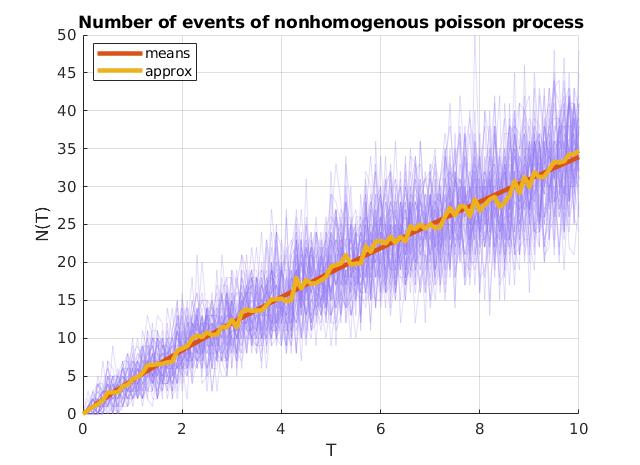
\includegraphics[width=0.7\textwidth]{bilder/task3_events.jpg}
%     \caption{Plot over the number of events of 50 processes over different times, with theoretical and estimated means overlaid.}
%     \label{fig:t3events}
% \end{figure}

\begin{figure}[H]
    \centering
    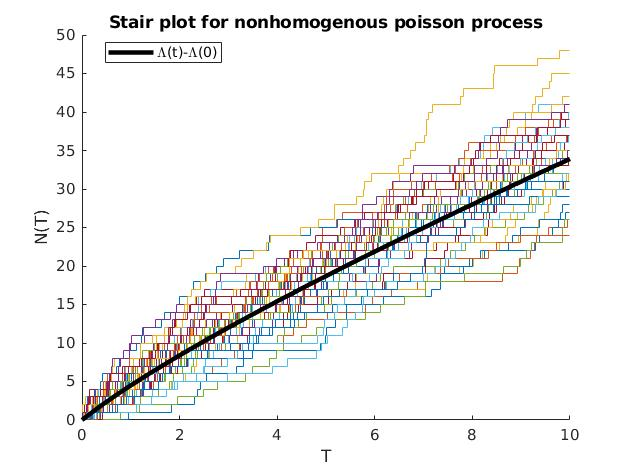
\includegraphics[width=0.7\textwidth]{bilder/task3_trajectories.jpg}
    \caption{Stair plot over 50 poisson processes over time.}
    \label{fig:t3stair}
\end{figure}

Running the simulation for $N = 100\ 000$ (with each $T = 10$) we get the following result:
\begin{verbatim}
  Approximative mean: 33.912
  Approximate variance: 33.580
\end{verbatim}
\label{res:ex3c}
We see that this corresponds well to the theoretical value of them both: $\Lambda(T) - \Lambda(0) = \mu = \sigma^2 \approx 33.900$
% TODO: actually \lambda_N + \Lambda(T) - \Lambda(0) ?

\subsection{Conclusions}
\label{sec:conc3}
The simulated process seems to follow the values expected from the theoretical formulas.
This indicates that the algorithms works as intended giving an accurate simulation of the posed distribution.


% Reflect upon the results you have obtain.  
% How does the results relate to the main question and formulation of the task. 

% =========================== APPENDIX ===========================
\newpage
\appendix

%\section{Appendix}
%\label{sec:appendix}

\clearpage
